\documentclass{article}
\usepackage[spanish]{babel}
\usepackage[utf8]{inputenc}
\usepackage{tikz}
\usepackage{johd}

\title{Tema 2. Protocolo HTTP}

\author{José Antonio Fajardo Naranjo \\
	\small
	\tt{fajardonaranjoja@gmail.com} \\
	\date{}
}

\begin{document}
	\maketitle
	\begin{abstract} 
		\noindent Estos apuntes pertenecen al tema 2 de la asignatura Desarrollo Web en entorno servidor impartida en el 2ndo curso de FPGS de Desarrollo de aplicaciones web en el IES Martín Rivero durante el curso 2023/2024.
	\end{abstract}
	\newpage{\ }
	\tableofcontents
	\newpage{\ }
	\thispagestyle{empty}
	
	


	\section{Introducción}
	
	\paragraph{}El protocolo HTTP busca la simpleza y la eficacia para el intercambio de documentos. Aunque su uso principal es el intercambio de los documentos de hipertexto se puede usar para transferir otro tipo de elementos.
	
	\subsection{Funcionamiento}
	
	\paragraph{}El principio en el que se basa este protocolo es el tándem pregunta/respuesta. El cliente genera una pregunta con la forma de una petición HTTP que contiene, al menos, los datos que permiten identificar el recurso que le ha sido solicitado por el cliente. Esta petición no es más que un bloque de texto que viaja del cliente al servidor. Se compone de dos partes separadas por una línea en blanco (retorno de carro o salto de línea). La primera parte es la cabecera de la petición HTTP, que es obligatoria, mientras que la segunda es el cuerpo, que es opcional, dependiendo su aparición del tipo de petición HTTP. La línea en blanco ha de aparecer siempre, siendo completamente \textbf{obligatoria}. La respuesta mantiene el mismo formato de las peticiones.
	
	\paragraph{}Una respuesta HTTP sólo existe si se ha enviado previamente una petición HTTP al servidor, no tomando este último la iniciativa de enviar datos que no han sido solicitados por el cliente (con la tecnología de los \textbf{WebSockets} esto no es necesario, los servidores actualizan en tiempo real sin necesidad de petición).
	
	\paragraph{}El protocolo TCP se utiliza para el transporte de los bloques de texto de petición y respuesta HTTP. Por defecto, esta conexión mediante TCP se establece para cada par petición/respuesta. Sin embargo, la versión 1.1 propone una solución para transportar varios pares petición/respuesta con la misma conexión TCP. A continuación, encontramos el ejemplo utilizado en clase de paquete capturado.
	
	\begin{figure}[H]
		\centering
		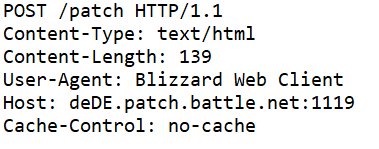
\includegraphics[scale=0.5]{images/peticionhttp.PNG}
		\caption{\label{fig1}Captura de una petición HTTP}
	\end{figure}
	
	\begin{figure}[H]
		\centering
		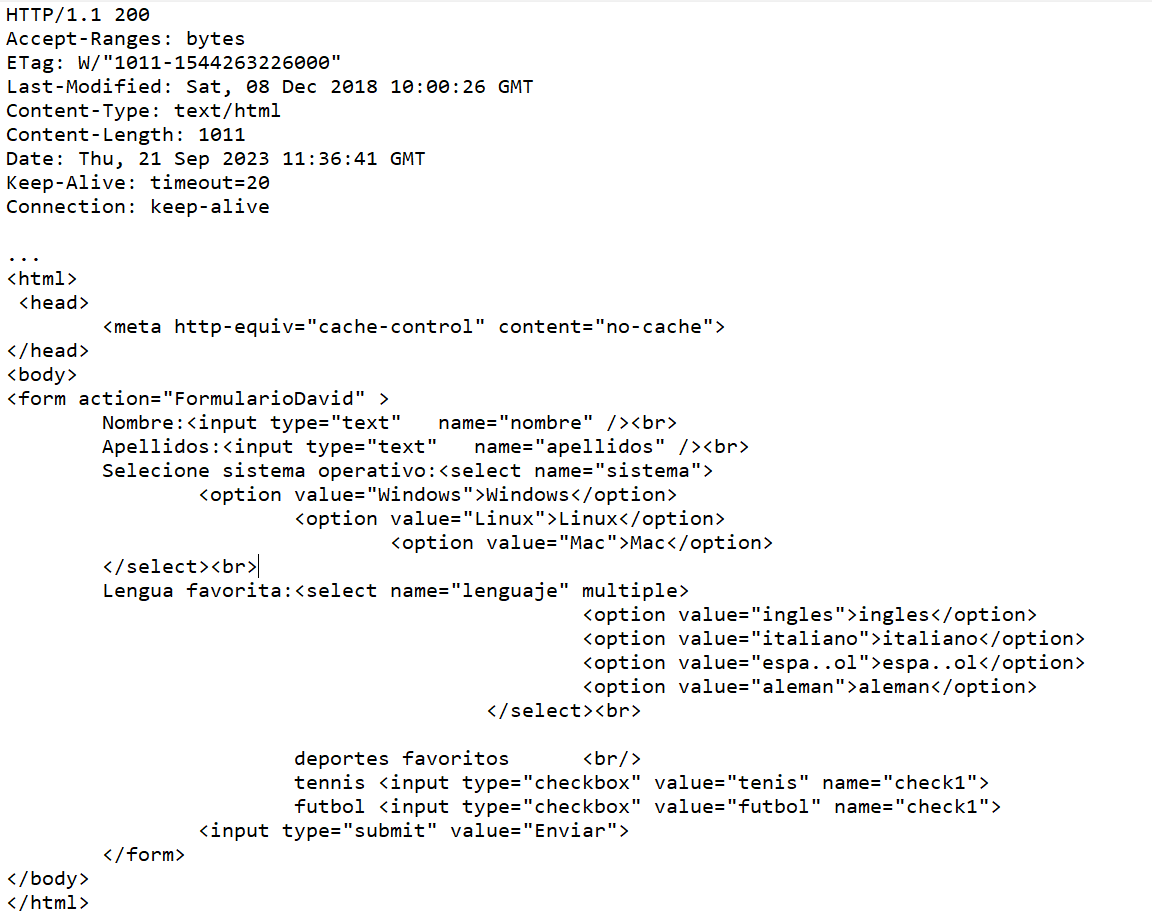
\includegraphics[scale=0.5]{images/respuestahttp.png}
		\caption{\label{fig2}Captura de una respuesta HTTP}
	\end{figure}
	
	\subsection{Las URL}
	
	\paragraph{}Las URL (Uniform Resource Locator) permiten localizar los recursos que se desean recuperar mediante peticiones HTTP. Se componen de una cadena de caracteres de cinco campos. Se ha de seguir el siguiente formato:
	
	\begin{center}
			\texttt{protocolo://identificador del servidor:número de puerto/recurso?parámetros}
	\end{center}
	
	\begin{itemize}
		\item Protocolo: indica el protocolo utilizado para el acceso al recurso. Nosotros usaremos HTTP aunque hay otros como FTP o mailto.
		\item Identificador del servidor: esta parte permite localizar el servidor en la red. Normalmente es el FQDN (Fully Qualified Domain Name), el nombre de dominio del servidor, que no da lugar a ambigüedades. Se tiene que transformar en la dirección IP para que el protocolo TCP pueda establecer una conexión con el servidor, de lo cual se encarga un servidor DNS (Domain Name System). Se puede usar una IP en la URL pero es más sencillo el FQDN.
		\item Número de puerto: este dato es el número de puerto TCP con el que se debe establecer la conexión. Este número funciona para que el protocolo TCP identifique una aplicación particular en una máquina. Este sistema permite el alojamiento de más de una aplicación por servidor. El puerto 80 es el que se asigna por defecto al protocolo HTTP.
		\item Recurso: esta parte de la URL permite determinar el recurso que se desea obtener. Puede estar compuesto por varios elementos separados por el carácter.
		\item Parámetros: son los datos que pasamos cuando la petición HTTP se hace, por ejemplo, sobre un recurso dinámico. Aparecen de la forma nombreDeParam=valorDeParam. Con el carácter \& se pueden separar estos parámetros.
	\end{itemize}
	
	\paragraph{}A continuación se muestran equivalencias entre los caracteres y su valor en ASCII, ya que algunos caracteres tienen una función en las URL:
	
	\begin{table}[H]
		\centering
		\begin{tabular}{|l|l|}
			\hline
			\multicolumn{1}{|c|}{\textbf{Carácter}} & \multicolumn{1}{c|}{\textbf{Codificación}} \\ \hline
			Espacio                                 & \%20 o a veces +                           \\ \hline
			"                                       & \%22                                       \\ \hline
			\%                                      & \%25                                       \\ \hline
			\&                                      & \%26                                       \\ \hline
			+                                       & \%2B                                       \\ \hline
			.                                       & \%2E                                       \\ \hline
			/                                       & \%2F                                       \\ \hline
			?                                       & \%3F                                       \\ \hline
			'                                       & \%60                                       \\ \hline
		\end{tabular}
	\end{table}
	
	\section{Las peticiones HTTP}
	
	\paragraph{}Las peticiones HTTP comienzan el diálogo entre un navegador (cliente) y un servidor Web. El navegador, por norma general, construye la petición HTTP en función de los datos contenidos en una página HTML. Todas las cabeceras de una petición comienzan por una línea con el mismo formato, contiene el tipo de la petición HTTP seguido del identificador del recurso solicitado y finaliza con la versión del protocolo HTTP (HTTP/1.1).
	
	\subsection{Los distintos tipos de petición}
	
	\paragraph{}La versión 1.0 del protocolo HTTP disponía de 3 tipos de petición HTTP:
	
	 \begin{itemize}
	 	\item GET: permite obtener un recurso disponible en el servidor. Es el tipo que se genera por defecto. No tiene ningún tipo de dato en el cuerpo de la petición y si necesita enviar parámetros al servidor se añaden a continuación de la URL.
	 	\item POST: se destina al envío al servidor de datos recopilados en formularios HTML. Presenta ventajas con respecto al método GET.
	 		\subitem No hay límite teórico de cantidad de información que se envía, porque se inserta en el cuerpo de la petición en lugar de en la cabecera.
	 		\subitem No se ven los datos en la barra de dirección del navegador, por lo cual existe más privacidad.
	 	\item HEAD: funciona como la petición GET, salvo porque el servidor no devuelve nada en el cuerpo de la respuesta HTTP. Los navegadores lo utilizan para la gestión del almacenamiento en caché de datos.
	 \end{itemize}
	
	\paragraph{}La versión 1.1 de protocolo HTTP añade nuevos tipos de petición.
	
	\begin{itemize}
		\item La petición PUT permite enviar un recurso al servidor para que éste lo guarde de forma permanente.
		\item La petición DELETE permite solicitar la eliminación de un recurso determinado.
		\item La petición TRACE permite solicitar al servidor la devolución en el cuerpo de la respuesta HTTP de una copia de la petición HTTP que acaba de recibir.
		\item La petición OPTIONS permite obtener datos sobre las opciones que se pueden utilizar para obtener un recurso.
	\end{itemize}
	
	\subsection{Las cabeceras de petición}
	
	\paragraph{}El cliente (navegador) añade las cabeceras de petición en el momento en que construye la petición HTTP. Cada tipo de navegador construye y ordena la cabecera de la petición HTTP de manera diferente. La función de estas es la de proporcionar al servidor información adicional acerca de la petición. Hay algunas que se consideran estándar y aparecen en todas las peticiones. Entre las más comunes se destacan:
	
	\begin{itemize}
		\item \texttt{Accept}: esta cabecera permite indicar al servidor qué tipos de datos se aceptan como respuesta. El formato en el que se tienen que indicar este tipo de datos es el MIME (Multipurpose Internet Main Extensions). Si el navegador no tiene ninguna preferencia, puede añadir la cabecera siguiente:
		\begin{center}
			\texttt{Accept: */*}
		\end{center}
		\item \texttt{Accept-Charset}: esta cabecera indica las preferencias respecto al juego de caracteres que puede usar el servidor para construir la respuesta HTTP. Ejemplo:
		\begin{center}
			\texttt{Accept-Charset: ISO-8559-1,utf-8}
		\end{center}
		\item \texttt{Accept-Encoding}: esta cabecera indica al servidor en qué lengua prefiere obtener el recurso solicitado. Ejemplo:
		\begin{center}
			\texttt{Accept-Language: es,en}
		\end{center}
		\item \texttt{Connection}: esta cabecera es de la versión 1.1 de HTTP. Determina cómo se comportarán las conexiones TCP utilizadas para la petición y la respuesta. Si el navegador desea mantener la conexión abierta puede añadir valor keep-alive para la cabecera. Por el contrario, con el valor close la conexión se cierra. Ejemplo:
		\begin{center}
			\texttt{Connection: keep-alive}
		\end{center}
		\item \texttt{Host}: esta cabecera de la versión 1.1 del protocolo HTTP especifica el FQDN (Fully Qualified Domain Name) y el número del puerto del servidor que aloja el recurso solicitado. Este nombre puede corresponder a un servidor físico o a uno virtual. Siempre es necesario que pueda transformarse en una dirección IP para que el protocolo TCP pueda transportar la petición HTTP. En caso de que se usen servidores virtuales hay varios FQDN con la misma dirección IP. La referencia hacia el servidor virtual adecuado se realiza con esta cabecera. 
		\begin{center}
			\texttt{Host: www.eni-ecole.fr}
		\end{center}
		\item \texttt{Referer}: esta cabecera contiene la URL del documento a partir del cual la petición HTTP ha sido generada. Se informa cuando una petición HTTP se construye después de la activación de un enlace de hipertexto o de la validación de un formulario. Ejemplo:
		\begin{center}
			\texttt{GET /index.php HTTP/1.1\\
			Referer: http://www.eni-ecole.fr/}
		\end{center}
		\item \texttt{User-Agent}: esta cabecera permite identificar el tipo de navegador en el origen de la petición, pudiendo utilizarse para realizar estadísticas o permitir al servidor optimizar el código enviado en función del tipo de navegador (especie de firma del navegador). Ejemplo:
		\begin{center}
			\texttt{User-Agent: Mozilla/4.0 (compatible; MSIE 7.0; Windows NT 6.0;\\
			SKCC1; .NET CLR 2.0.50727; InfoPath.2; .NET CLR 3.5.21022; .NET\\
			CLR 1.1.4322; .NET CLR 3.5.30729; .NET CLR 3.0.3061)}
		\end{center}
	\end{itemize}
	
	\section{Las respuestas HTTP}
	
	\paragraph{}Después de la recepción y tratamiento de una petición HTTP, el servidor genera una respuesta HTTP para transmitir el recurso solicitado al cliente. La estructura de esta respuesta es similar a la de la petición HTTP. Se compone de dos partes, la cabecera y el cuerpo, que se separan por una línea en blanco. También hay respuestas sin cuerpo. La primera línea de la parte de la cabecera ejerce una función específica debido a que esta línea se dedica al estado de la respuesta, definiendo el tipo de la misma, gracias al valor numérico correspondiente al código de estado de la respuesta que tiene en su interior.
	
	\subsection{Tipos de respuestas HTTP}
	
	\paragraph{}Las respuestas se organizan en 5 categorías según la primera cifra del código de estado. A continuación se muestran las distintas categorías y los más vistos de cada una de ellas:
	\begin{itemize}
		\item \textbf{1XX}: información.
			\subitem \textbf{\textit{100 continúa}}: el servidor genera esta respuesta cuando recibe una petición HTTP en varias partes. El cliente necesita esta respuesta para saber que el comienzo de la petición se ha recibido satisfactoriamente y que el servidor está a la espera de continuación.
		\item \textbf{2XX}: éxito.
			\subitem \textbf{\textit{200 OK}}: ésta es la respuesta más frecuente generada por los servidores, indica que se ha tratado correctamente la petición.
			\subitem \textbf{\textit{201 creado}}: es generada por el servidor cuando se ha creado un recurso correctamente en el servidor mediante una petición HTTP de tipo PUT.
			\subitem \textbf{\textit{204 sin contenido}}: es generada por el servidor cuando genera una respuesta sin cuerpo, es decir, solamente con cabecera de respuesta HTTP.
		 \item \textbf{3XX}: redirección.
		 	\subitem \textbf{\textit{301 movimiento permanente}}: el recurso solicitado por el cliente se encuentra ahora en otra ubicación, que se indica en la cabecera ``location''.
		 	\subitem \textbf{\textit{302 movimiento temporal}}: el recurso solicitado por el cliente se encuentra temporalmente en otra ubicación, devuelta en un enlace de hipertexto hacia la nueva ubicación.
		 	\subitem \textbf{\textit{304 sin modificar}}: es generada por el servidor al recibir una petición condicional del cliente, indicando que el recurso presente en el servidor es idéntico al que ya está disponible en el cliente.
		 \item \textbf{4XX}: error provocado por el cliente.
		 	\subitem \textbf{\textit{400 petición incorrecta}}: la sintaxis de la petición HTTP es incorrecta.
		 	\subitem \textbf{\textit{401 no autorizado}}: el acceso al recurso solicitado requiere la autenticación del cliente.
		 	\subitem \textbf{\textit{403 acceso prohibido}}: el acceso al recurso está prohibido.
		 	\subitem\textbf{\textit{404 no encontrado}}: el recurso solicitado no se ha encontrado.
		 	\subitem \textbf{\textit{405 método no admitido}}: este tipo de petición HTTP utilizado para acceder al recurso no está admitido.
		 	\subitem \textbf{\textit{407 autenticación proxy}}: un servidor proxy envía este tipo de respuesta cuando requiere la autenticación del cliente antes de transmitir la petición a un servidor.
		 \item \textbf{5XX}: provocado por el servidor.
		 	\subitem \textbf{\textit{500 error interno del servidor}}: un problema de funcionamiento impide al servidor tratar con éxito la petición.
		 	\subitem \textbf{\textit{503 servicio no disponible}}: una sobrecarga del servidor impide tratar la petición.
		 	\subitem \textbf{\textit{505 versión HTTP no compatible}}: el servidor no puede utilizar la versión del protocolo HTTP especificada en la petición.
	\end{itemize}
	
	\subsection{Las cabeceras de respuesta}
	
	\paragraph{}El servidor genera las cabeceras de respuesta cuando construye la respuesta HTTP. Cada tipo de servidor tiene su propia técnica para construir una respuesta HTTP y las cabeceras no son necesariamente las mismas entre servidores. Hay un conjunto que bien se puede llegar a considerar estándar y aparecen prácticamente siempre en una respuesta HTTP. Las cabeceras se usan principalmente para proporcionar al navegador información adicional acerca de la respuesta. A continuación se muestran las más frecuentes:
	
	\begin{itemize}
		\item \texttt{location}: esta cabecera de respuesta se encuentra en respuestas HTTP de redirección (3XX) para indicar la nueva ubicación donde se encuentra el recurso solicitado.
		\item \texttt{server}: esta cabecera de respuesta contiene información acerca del tipo de servidor que ha generado la respuesta.
		\item \texttt{via}: esta cabecera de respuesta se añade a la respuesta de origen realizada por el servidor cuando la respuesta ha pasado por un servidor proxy.
		\item \texttt{retry-after}: esta cabecera de respuesta se encuentra principalmente en las respuestas HTTP de tipo 503 (servicio no disponible) para indicar la duración estimada de la no disponibilidad del servidor. Esta duración se expresa en segundos de espera o con una fecha y hora a partir de la cual el cliente podrá reformular la petición.
		\item \texttt{proxy-authenticate}: este tipo de cabecera es incluida por un servidor proxy en una respuesta HTTP 407. Indica el método de autenticación esperado por el servidor proxy. El navegador utiliza esta información para reformular la petición que contiene los datos de autenticación del usuario, añadiendo la cabecera de la petición proxy-authorization con los datos del usuario a la cabecera de la nueva petición que ha generado.
		\item \texttt{allow}: este tipo de cabecera se encuentra en las respuestas HTTP 405 (método no admitido) para indicar los métodos HTTP aceptados para acceder a un recurso determinado.
		\item \texttt{connection}: esta cabecera es de la versión 1.1 del protoclo HTTP. Indica cómo se tiene que gestionar la conexión TCP una vez el cliente ha recibido la respuesta.
		\item \texttt{content-encoding}: esta cabecera indica el método de compresión utilizado por los datos contenidos en el cuerpo de la respuesta HTTP.
		\item \texttt{content-language}:esta cabecera indica el idioma del documento contenido en el cuerpo de la respuesta HTTP
		\item \texttt{content-length}: esta cabecera indica el número de bytes contenidos en el cuerpo de la respuesta HTTP.
		\item \texttt{content-MD5}: esta cabecera permite la verificación de la integridad del contenido de la respuesta. La firma MD5 calculada por el servidor sobre el cuerpo de la respuesta se añade a continuación de la misma con esta cabecera. El cliente realiza la misma operación cuando recibe la respuesta y compara los resultados para comprobar una posible alteración de la respuesta durante la transferencia.
		\item \texttt{content-type}: esta cabecera indica el tipo MIME (Multipurpose Internet Mail Extensions) del documento contenido en la respuesta. Ciertos navegadores la necesitan para poder interpretar correctamente la respuesta, que si no está hace que se trate la respuesta como texto en bruto.
		\item \texttt{date}: esta cabecera contiene la fecha y la hora de generación de la respuesta HTTP.
		\item \texttt{last-modified}: esta cabecera contiene la fecha y la hora de la última modificación del recurso en el servidor.
		\item \texttt{WWW-authenticate}: este tipo de cabecera se incluye en las respuestas HTTP 401 (no autorizado) para reclamar al cliente los datos de su identidad. Por norma general, los navegadores muestran automáticamente un cuadro de diálogo que permite al usuario introducir un nombre y contraseña, siendo la validación de este cuadro la que provoca nuevamente el envío de una petición HTTP hacia el servidor con los datos recopilados.
	\end{itemize}
	
	\section{Gestión del almacenamiento en caché}
	
	\paragraph{}Generalmente en una aplicación, el contenido de algunos recursos cambia con muy poca frecuencia. Para optimizar las transferencias entre cliente y servidor, el navegador puede almacenar temporalmente estos recursos. Cuando tiene que realizar de nuevo una petición HTTP para obtener uno de estos recursos, puede usar la versión que ha almacenado localmente en vez de contactar de nuevo con el servidor, no sin antes asegurarse previamente de que la versión del recurso que mantiene localmente es válidad. Con técnicas como la petición condicional o la realización previa de una petición HEAD para obtener la parte de la cabecera de la respuesta HTTP por parte del servidor.
	
	\subsection{Gestión realizada por el cliente}
	
	\paragraph{}Hay varias cabeceras de petición HTTP para darle un carácter condicional a una petición HTTP. Lleva generalmente una fecha o identificador asociado al recurso.
	\paragraph{}La primera solución para el navegador consiste en añadir la cabecera if-modified-since seguida de la fecha y hora de creación del recurso que ya tiene en caché. De este modo, solicita al servidor que le transfiera el recurso si ha sido modificado posteriormente a esta fecha. Si es el caso, el servidor devuelve al cliente el recurso en una respuesta HTTP 200. Si el recurso no se ha modificado en el servidor desde esa fecha, éste genera una respuesta HTTP 304 y el navegador utiliza la versión del recurso que ya tenía en la memoria caché.
	
	\paragraph{}La segunda solución usa además una etiqueta asociada por el servidor al recurso, modificando este último el valor de la etiqueta en cada modificación del recurso.
	
	\paragraph{}Para generar este tipo de petición, el navegador añade la cabecera if-none-match seguida de la etiqueta correspondiente a la versión del recurso que tiene en caché. Como sucede con la anterior solución, el servidor devuelve al cliente el recurso si no tiene la misma versión, si por el contrario la tiene, genera una respuesta HTTP 304.
	
	\subsection{Gestión realizada por el servidor}
	
	\paragraph{}El servidor es el encargado de añadir a la cabecera de la respuesta la información necesaria. Esta información se transmite con las siguientes cabeceras:\\
	
	\begin{itemize}
		\item \texttt{date}: esta cabecera contiene la fecha y hora de generación de la respuesta HTTP. El navegador la utiliza como referencia para realizar peticiones HTTP condicionales.
		\item \texttt{Etag}: esta cabecera representa el valor de la etiqueta asociada por el servidor al recurso cuando se transmite al cliente.
		\item \texttt{expires}: esta cabecera se indica al navegador hasta cuando puede conservar en caché el recurso enviado. Cuando termina ese tiempo, el navegador tiene que realizar una nueva petición HTTP si necesita usar el recurso de nuevo.
	\end{itemize} 
	
	\paragraph{}El servidor también puede impedir el almacenamiento en caché de un recurso por el navegador añadiendo la cabecera de respuesta \texttt{cache-control} con el valor \texttt{no-cache}
	
	\paragraph{}Se explica todo de manera más detallada en la norma RFC2616.
\end{document}